%!TEX root = ../tommaso-thesis.tex
%!TEX spellcheck = en_US


% \chapter{Sympathy for the Devil:\\Reified Collection of Runtime Errors}\label{ch:reified}
\coolchapter{Sympathy for the Devil}{Reified Collection of Runtime Errors}{ch:reified}


Software development involves iterations of writing, running, testing, and debugging code.
When fixing a defect, developers construct a mental model of the system that explains the defect and eventually identifies its cause.
However, filtering complete, coherent, and reliable information from a running system is not an easy task: Using a simple approach, like generic logging, is often ineffective because it deconstructs and flattens the state into textual data, thus requiring ad-hoc understanding and processing.
On the other hand, collecting structured information in form of objects to observe and understand a precise property of the system requires specialized ad-hoc code, decoupled from the system's domain, and is usually not reusable.

We concluded \chref{ch:stacktraces} by saying that collecting stack traces can teach us stories about the system that we hardly would have noted otherwise.
In this chapter generalize the approach by presenting a domain-specific data collection framework that enables the developers to extract selected information about a system.
The developer is able to take a snapshot of all the information deemed relevant about a piece of code by writing few lines of code, thus enabling structured and effective logging and reporting of errors.
We detail our framework in the context of a bug reporting platform, and illustrate how such an approach can be used to create in-depth and reliable domain-specific bug reports.

\structure

%\secref{sec:reified-related} illustrates  the state of the art about collecting information on defective software states.
\secref{sec:reified-framework} describes the approach from a conceptual point of view together with its requirements, while \secref{sec:reified-implementation} illustrates the architecture and implementation of the proposed approach.
In \secref{sec:reified-stories} we assess the technique through three stories that illustrate how our approach can support development and debugging.
Finally, \secref{sec:reified-summary} concludes the chapter and outlines directions for future work.



%%%%%%%%%%%%%%%%%%%%%%
\section{The Tools We Use To Develop} \label{sec:reified-introduction}
%%%%%%%%%%%%%%%%%%%%%%

Computer systems have become pervasive in many human activities, where the high penetration of machine-controlled devices led to a tremendous increase in the complexity of the involved software.
This phenomenon turned modern software development into a multifaceted activity, where a one-developer team is no longer a viable option: Building software is above all a collaboration and communication activity.
Writing code is only a small part of the process: Several phases such as design, testing, and maintenance, play a role as fundamental in the success of a project.
In fact, maintenance often represents a significative percentage of a developer's time: Researchers showed that the effort put in reading and understanding code outweighs the effort needed to write it~\cite{Corb1989,Fjel1983,Zelk1979,Mine2015b}.
In such a scenario, one would imagine that the effort for providing means to aid developers would focus on refined tools to navigate, understand, and inspect the code.
While this is partly true, many of the modern editors and IDEs put the biggest accent on how developers write code, leaving program comprehension as a secondary task that is implicitly more complicated.


\subsubsection{The Curse of Text}

It is easy to see why understanding software is hard: Reading code requires reading text that contains structured information in a language that does not follow the same logic of natural language.
To understand a fragment of code, a developer has to mentally parse a source file, identify and extract the necessary information, and build a \emph{mental model} of the (intended) behavior of the software.
The same process happens when printing log messages to expose the state of the system: Log messages embody fragments of information that the developer has to fit into her mental model, and use it to reverse engineer the source of an error by trial and error.

To ease this process, both researchers and industry built a plethora of tools like debuggers and code inspectors, that allow developers to run a program in a controlled environment, and to check the internal status of its variables.
Other tools, like code browsers, support fast linking between the entities in the code, while loggers allow to print and store useful runtime information.
Finally, test suites allow to define a set of expected behaviors, and to constantly check if any of these rules is satisfied.

All these tools however do not change the fundamental way we interact with the code: Eventually, the developer needs to read the code, and therefore undergo the process of building its mental model.
This is because all these tools rely on the same, strong, underlying assumption: Source code is text, therefore the tools we are using to interact with it are shaped around text editing tools.
This assumption reflects the way we use to store our programs, \ie plain-text files containing the declaration of our models.

We propose a novel approach for runtime data collection: We advocate the use of objects to store information about an exception, in order to preserve the multidimensional nature of the information, and leverage the implicit properties that can be obtained by the data structure.
By describing errors as first-class citizens of a system, and using a storage format that does not flatten the information, we can reify logs and leverage their expressive power to support a number of development activities.
A structured data source allows to build a set of specialized tools to browse the data in an incremental fashion, to discover its implicit structure, or to enable the use of automated analysis, mitigating the need of a data cleaning phase.
It can also be stored and sent for debugging purposes, thus creating bug reports with a much higher level of detail and reliability than simple plain text.


% %%%%%%%%%%%%%%%%%%%%%%
% \section{Related Work} \label{sec:reified-related}
% %%%%%%%%%%%%%%%%%%%%%%
%
% Several tools in both academic and industrial contexts use the vast amount of data generated during the development and debugging process to enable a number of different analyses.
% Many aspects of development can benefit from leveraging this data, but among them it is interesting to consider two main areas especially oriented toward supporting software development: bug \emph{fixing}, and \emph{visualization} for program comprehension.
%
% \subsection{Fixing Bugs}
%
% The first major development activity that benefits from runtime data is bug fixing.
% The purpose of the research in this area is to support and automate the identification of the portions of code that contain an error, thus alleviating the developer from the burden of walking through the whole execution path to localize the cause of a bug.
%
% Several approaches use techniques to gather system information and detect errors in an automated fashion.
% For example, researchers collected large volumes of stack traces to identify patterns in the errors of a system, to assist the early detection of new problems or regressions, and to build a knowledge base of common problems~\cite{Han2012,Arno2007,DalS2015b}.
% Zimmermann \etal performed a survey asking developers about the challenges they have to undergo while dealing with bug reports, finding that one of the biggest problem comes from the reliability of the reported data~\cite{Zimm2010a}, hinting at the need for an automated approach that collects meaningful data.
%
% Cleaning the data in log files is also an issue when inspecting the data, or while performing analyses.
% For example, Aye proposed a preprocessing stage to overcome the problem of huge log files in web applications, with the purpose of cleaning the data to allow a subsequent mining step~\cite{Aye2011}.
%
% \subsection{Comprehension and Visualization}
%
% Researchers also used the massive amount of data produced by the execution of a system to create a view of the system at a global level, to detect hidden interactions or unexpected patterns and give an overview of the system.
%
% For example, Koike proposed a tool to visualize log files of the Snort\footnote{\url{https://www.snort.org/}} intrusion detector and assist system administrators to identify intrusion attempts in a system~\cite{Koik2004}.
% Moreta and Telea visualized log files using hierarchical clustering to uncover patterns of interest, with the purpose of monitoring dynamic allocation of memory and support the analysis of software repositories~\cite{More2007}.
%
% Orso \etal proposed a tool to monitor the logs of deployed software by means of visualizations generated by data mining techniques applied on runtime execution data~\cite{Orso2003}.
% De Pauw \etal built a tool to visualize the execution of Java programs, with the purpose of aiding the developer to understand the execution of the program and identify problems like performance bugs~\cite{De2002}.
%
% The approach by Dal Sasso \etal collected data from different data sources, and combined them to create a high level view of the usage of the system~\cite{DalS2015b}.
% They showed that large amount of logging data and user interaction data can show hidden paths of usage of the entities of the system.
%
% Finally, researchers also tried approaches to improve the textual representation of software artifacts by augmenting their description with a markup language~\cite{Badr2000,Male2002a}.
% While these approaches are focused on describing source code, they are still relevant for program comprehension to support bug fixing, as they explicitly render the properties that are hidden in the textual form of the source code.


%%%%%%%%%%%%%%%%%%%%%%%%%%%%%%%%%%%%%%%%%%%%
%%%%%%%%%%%%%%%%%%%%%%%%%%%%%%%%%%%%%%%%%%%%
\section{A Domain-Specific Reporting Engine} \label{sec:reified-framework}
%%%%%%%%%%%%%%%%%%%%%%%%%%%%%%%%%%%%%%%%%%%%
%%%%%%%%%%%%%%%%%%%%%%%%%%%%%%%%%%%%%%%%%%%%

In this section we outline our approach for collecting information about runtime errors.
We explain the benefits of collecting this runtime data and show how and why development can benefit from modeling this information.
The final goal is to integrate the resulting framework into a modern development environment, to enable smooth and descriptive fruition of debugging information, and to provide the groundwork for building interactive tools that present the data in a meaningful context.

\subsection{Who Needs Models?}

The purpose of a programming language is to equip the developers with the means to communicate, both to a machine and to other people, the intended behavior of a program.
Therefore, we can view a program  as the crossroads between the high level intent of the developer and the machine language that details the steps needed to accomplish it.

Clinging to the idea of a language that feels natural to describe algorithms, developers kept using the tools used for text editing to also manage source code.
The large number of specialized tools that usually enrich the development experience in a text editor never evolved beyond its underlying representation, making writing source code mainly a string manipulation process.
Using the widely understood format of plain text has numerous advantages, but it has one major drawback: It employs a \emph{flat} format do describe structured data, thus losing track of several properties that have to be inferred.
This means that the information that is contained in the data is not directly accessible by the developer, but hidden in the underlying implicit structure that has to be rebuilt, for example with a parser.
Paraphrasing the allegory of the Cave of Plato, we are trying to learn the behavior of the entities in our system by looking at the shadows they project on the wall, represented by the textual representations~\cite{Plato380a}.

While the goal of this work is not to criticize how we represent source code, it still helps us to comprehend how a developer perceives software development, since the very beginning of her training.
Unsurprisingly, if we think about source code in terms of text, the natural consequence is to treat as text also the product of the execution of such code.
As a result, the majority of logging and bug reporting systems collect messages as lines of text, stored in a text file.

We can improve the way we deal with the information produced by a software system by employing a different approach, that captures the runtime data preserving its structure (\eg the structure of the involved objects at runtime) and allows to perform a finer grained analysis.
Changing how we deal with data means changing the representation we use to interact with it: We need to employ a model that does not flatten the data it describes, but that maintains a structured relationship with the information it is derived from.

To overcome the difficulties of dealing with plain text to analyze programs, researchers tried to employ different model to represent source code, like \textsc{srcML}~\cite{Male2002a} or \textsc{JavaML}~\cite{Badr2000}.

In a similar fashion, the Smalltalk programming language proposes a system to store and access its source code that differs significantly from the usual text file approach.
Smalltalk proposes an approach where the whole system is contained in a single file named {\em image}.
This file contains a serialized version of the core system, its libraries, its IDE and tools, the code that the user writes inside the system, and the entire execution state composed of the existing objects when the image is saved.
Therefore, the user does not write a program through a normal text editor, but uses the internal browser of the system to navigate its code, and can use \emph{inspectors} to examine objects at any time.
Using this approach allows Smalltalk to achieve full \emph{liveliness}, as the whole system (both the source code and the runtime) can be manipulated programmatically.
Inspired by the Smalltalk image example, there is no reason that prevents us to apply this approach to runtime generated data, to increase the capabilities of the development environment.

\subsection{Design of the Framework}\label{sec:reified-design}

We want to devise an approach for recording the behavior of an executing program in a structured and customizable way, thus creating a powerful logging system that can talk with objects to extract specific and structured information.

To extend the behavior of the logging system, the first step is to define a model to describe the data we want to observe and collect.
The goal of this model is to reify debug messages and store them to obtain a level of detail as near as possible to the original objects they are derived from, and to preserve all the information that describes the actual running system.


\subsubsection{Shape of the model}

The state of a running system is normally a significantly complex entity, with several possible combination of its variables: Providing a description that is both complete and easily understandable is not an easy task.

Usually, during a debugging session, the easiest approach to quickly understand an unexpected behavior is to verify the state of a program by retrieving data about one or more objects at runtime.
Developers usually perform this operation by either printing a log message, or by using an object inspector.

In both cases there is a fundamental problem: To isolate the error, the developer has to (1) identify an unexpected behavior, (2) select a set of properties to observe, (3) change the program to output these properties, and (4) correct the program accordingly.
Using this process implies that every change requires a new run of the system.

While this would not pose any hard consequence in trivial development scenarios, it might become a problem if the flow of the program is not fully deterministic, like in case of concurrency, or if it relies on user input.
Unfortunately, these cases are also the hardest to identify and correct, which would therefore require the most support by the debugging tools.
For example, in the case of a multithreaded application, different runs would result in different internal states: An error in the execution logic, like an unprotected access to a resource, would make an error to appear only under certain conditions, resulting in what is called an \emph{Heisenbug}~\cite{Grot2005}.

Another issue comes with the necessity of understanding and correcting the problems experienced by the users of a program.
Understanding the condition under which a specific error occurred, and reproducing it for fixing, is one of the hardest things in the debugging process, that consumes a considerable amount of time that could be spent to develop new features.
Since the developers do not have access to the original environment where the error originally occurred, they have to infer it from the description of the user, or from the textual logs generated by the system, if any.
Users, however, cannot be expected to have the necessary technical background to effectively report a bug, which leads to a problem in the reliability of the information that they report to the developers~\cite{Zimm2010a}.

Our goal is to have an explicit, flexible, and specific out-of-the-box model that allows developers to observe the state of the system quickly, reliably, and with the lowest effort.
The cognitive cost for building a mental model of a system takes a significative toll on the energy of developers.
This method however brings a constant cost inside the iterative process of understanding-and-correcting code, as building a mental model is a task that must be performed every time, and does not scale.
As such, we want to remove this cost.

We set the guidelines for designing such a framework for reified data collection as:

\begin{enumerate}
  \item\label{enum:object} whenever possible, we collect the original entity that is involved in the event that we are observing;
  \item\label{enum:simplify} when collecting the whole entity is not possible, we create and store a simpler representation;
  \item\label{enum:custom} we want our framework to be easily extendable and customizable;
  \item\label{enum:domain-specific} we should not collect data we are not interested in;
  \item\label{enum:privacy} we should be careful in handling possibly sensible data.
\end{enumerate}

The guideline (\ref{enum:object}) defines the main scaffolding of our approach: We are interested in collecting information from an entity in the system.
Therefore, there is no need to prematurely flatten the information that the entity conveys: We rather store the whole entity, and delay its serialization, waiting for future instructions on how to use the information.

There are, however, some cases where the whole entity is not suitable for reporting the information.
This is especially true with entities that might change their status for external causes, or entities that might expire, for example in the case of database connections, or short lived sessions in a multiuser system.

In some other cases, we might not want our collection to expose sensible data, like passwords or private source code, as detailed in guideline (\ref{enum:privacy}).
In this case, we apply the guideline (\ref{enum:simplify}): if it does not make sense to collect a piece of information, we anticipate the simplification process to create a safe copy of the original entity, and collect the cleaned version.
Of course, this is strictly connected to the application domain, and it is not possible to generalize all the possible cases where we do not want to collect specific data.
Guideline (\ref{enum:custom}) specifies that, to be effective, our framework must allow easy customization of its details.

As an example, consider the case where we want to monitor, from a logging perspective, the errors that users get while accessing a resource.
Usually, we would add a command to write a text line into a log file, to store the user and the action.
The more information we want to extract, the more text we have to print, with the effect of cluttering the log file.
Using the approach we defined, we can setup a rule that activates when the system generates an error that involves the user, and store the entity of the user (guideline \ref{enum:object}).
In this way, we can directly access the actual entity related to the user, query it about its associated session, and the information about the action that the user was trying to perform.
We can also avoid to collect data that we do not want to share, like the password (guideline \ref{enum:simplify}).

This allows us to have a conversation with the entities we are dealing with, rather that collecting some passive text, thus enabling the development and customization of interactive tools that empower the user with the ability of browsing the entities related to the error, and get a quicker and more reliable grasp of the status of the system during an error.


\subsubsection{Collectors}

We need a strategy to let the user of our framework describe its own custom data collection, to implement the flexibility required by our approach (guideline \ref{enum:custom}).

To address this aspect, we define the concept of \emph{collectors}: Small entities that describe how and when to observe a part of the system.
A collector has three main purposes:

\begin{enumerate}
  \item define how to collect some data;
  \item define when to collect some data;
  \item describe itself.
\end{enumerate}

The main purpose of the collector is to define the data of interest: It must describe what to select and what to discard.
For example, going back to the logging example, the system will pass some context to the collector, that will copy the user entity and remove the sensible data, like the password, or mask the username, if the purpose of the collection is to be sent remotely and published in a bug report.

Defining when to collect the data is the other crucial aspect of the framework.
We are defining an approach that customizes the data need for certain types of data, therefore defining a domain-specific data collection.
Collecting data pertaining to a user is meaningless if we are dealing with an error generated for example from a string.
That is why each collector has to know when to activate itself: the system passes the context of the error to the collector, which checks its internal activation rule to decide whether to trigger the collection or not.

Finally, in a scenario where several collectors are involved and activated automatically depending on the entities involved with the error, we need a description to tag the collected data and present it to the user in an informative manner.

By employing the mechanics of the collectors we can build a data collection framework that is fully customizable and that collects first-class, reified entities, to enable a domain-specific system monitoring framework.
Such a framework can be employed to replace normal logging messages with a detailed snapshot of the state of a program, that can be then browsed with interactive tools, or that can be employed to collect failure data an pack it for remotely reporting an unexpected behavior.
This remote reporting mechanism can be the first step towards a smarter bug reporting system, that allows a deep inspection of the state of a system, while preserving the privacy of its users.
Being able to define the context of the error is crucial for the success of the whole approach, as we can only operate on the data we can manipulate.


%%%%%%%%%%%%%%%%%%%%%%%%%%%%%%%%%%%%
%%%%%%%%%%%%%%%%%%%%%%%%%%%%%%%%%%%%
\section{Implementing The Framework} \label{sec:reified-implementation}
%%%%%%%%%%%%%%%%%%%%%%%%%%%%%%%%%%%%
%%%%%%%%%%%%%%%%%%%%%%%%%%%%%%%%%%%%

\begin{figure*}[ht]
  \centering
  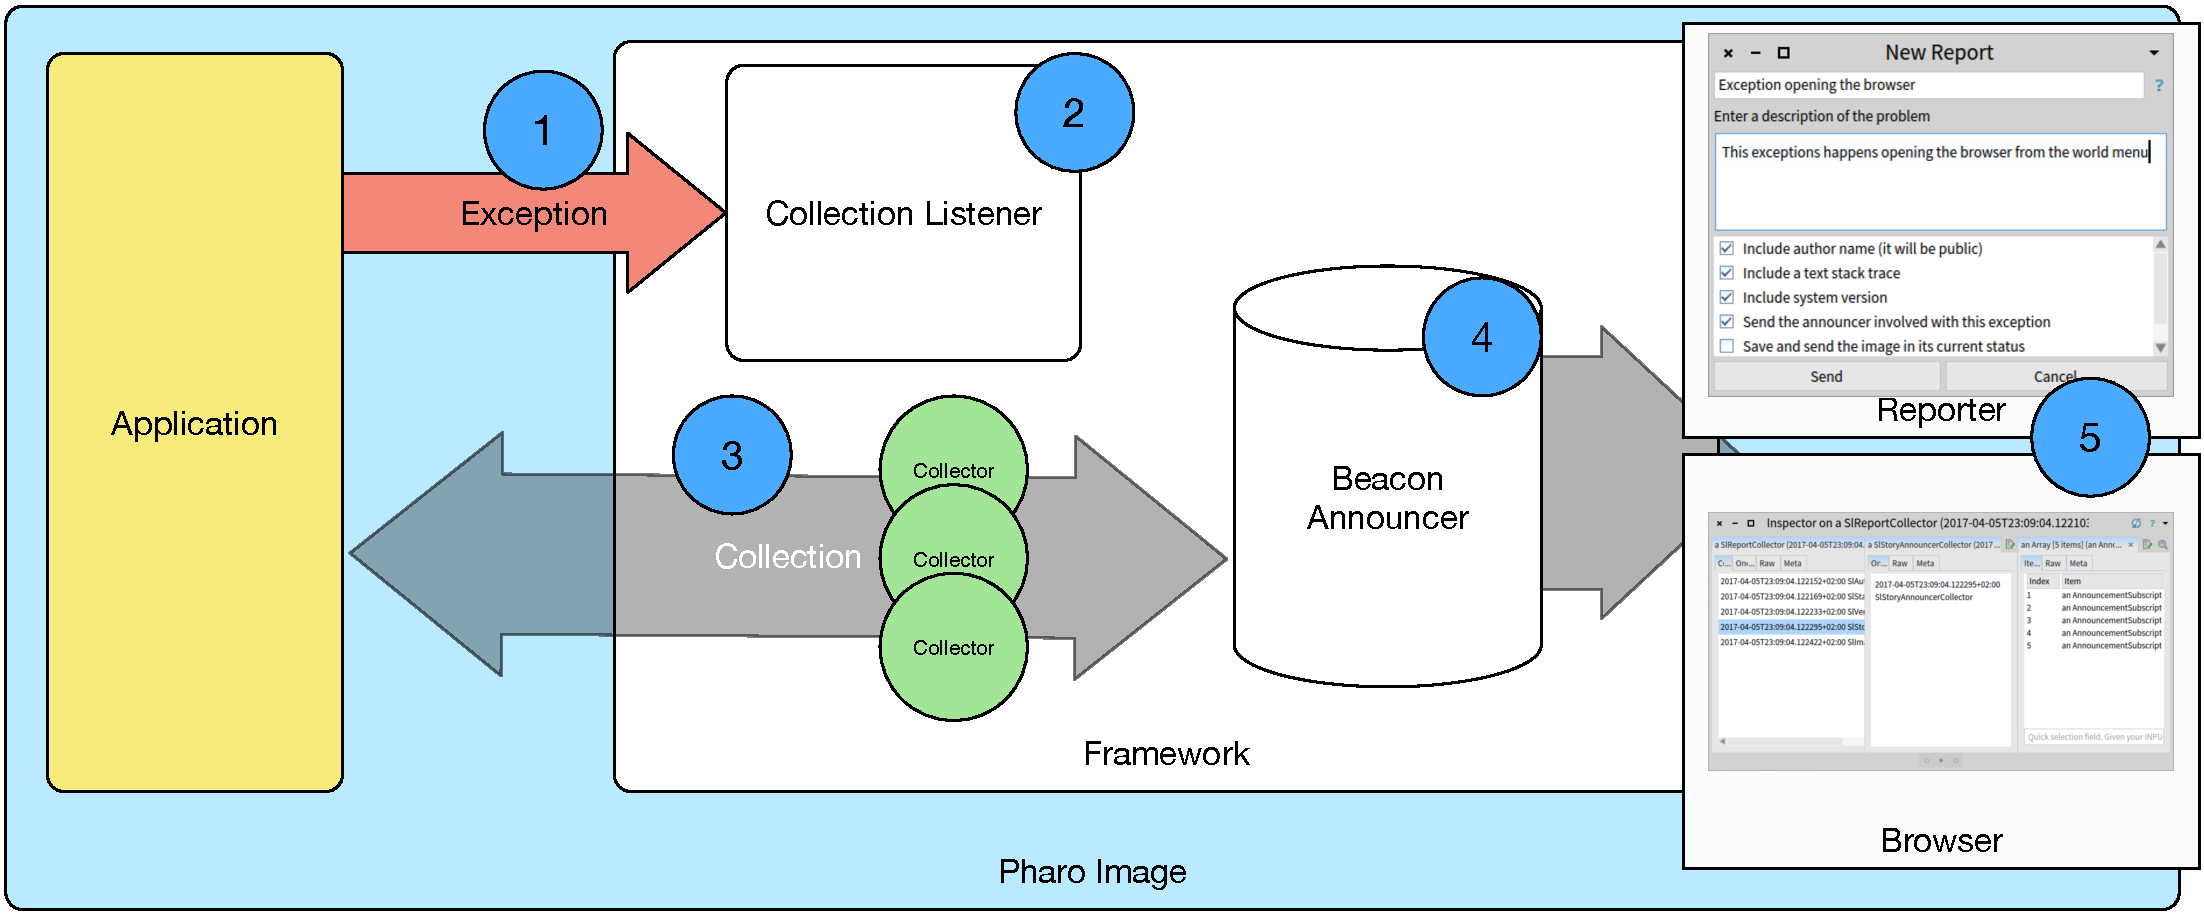
\includegraphics[width=.9\linewidth]{reified/process}
  \caption{The workflow to collect data using collectors, showing the architecture of \sln}
  \label{fig:architecture}
\end{figure*}

We now present the implementation details of the framework for the Smalltalk programming language, while \secref{sec:reified-summary} we will also discuss the challenges of generalizing such an approach to other programming languages.

In implementing our framework, we need to consider a number of aspects pertaining to the control of the system, first of all the ability to directly catch errors and manipulate its context to extract the relevant data in a usable state.
Accomplishing such a task is strongly dependent on the programming language of choice with the result that the amount of technical details that can be considered is humongous, and out of the scope of this work.
We implemented and test the effective feasibility of our approach using \pha.
The fact that the whole system is described using objects allows us to easily inspect faulty states of the system by interacting through the \texttt{Context} object, and simplifies the reification process of the interesting entities.

While the use of \pha enables full flexibility and control over the execution of a program, one may wonder whether this hinders the applicability of the approach to more general examples.
We believe that this does not affect the possibility to implement an analogous framework for a different programming language.
\secref{sec:reified-summary} contains a deeper discussion about the generalizability of our approach.

\subsection{Implementation Details}

The abstractions in the \pha environment concern the whole runtime of the system, allowing to inspect and manipulate it by querying objects.
The main benefit of \pha is that we can freeze the execution of a program, and easily access the whole system status at the moment of the interruption.

The principal element we are interested in is the \entity{thisContext} variable.
This special variable stores an instance of \entity{Context}, an object that mimics the behavior of an \textit{activation record} that contains all the information about the current execution of the program, such as the list of the variables in the scope, the method that is currently executing, the class that owns the method, the program counter of the line of code we are executing, and other information useful in describing the running session.


\subsubsection{Implementing Collectors}

We designed our framework around the idea of \emph{collectors}.
In \secref{sec:reified-design} we defined a collector as an entity that knows how and when to collect data, and that provides a description for this data.
By following the object-oriented nature of \pha we can implement a collector as a class.
While having a class for each collector might seem overkill, that might eventually bloat the system rather than supporting maintenance, it has the advantage of providing full control to the user of our framework, granting the flexibility to select the data she wants to observe.
The whole strategy can be encapsulated in a single class, thus decoupling the collector from the source code it is observing and providing a behavior that can be plugged and un-plugged seamlessly.

We define the class \entity{DataCollector}, that defines the template for implementing a collector.
A user can create a new collector by subclassing this class, and implementing four methods that define its behavior:

\begin{description}

\item \method{\#tag} --- the name of the method, used to reference the collected data by means of an automated approach;

\item \method{\#description} --- a short description of the data collected by the class, displayed to the user when presenting the data or when asking for permission to send the data to the issue tracking system;

\item \method{\#when:} --- an expression that evaluates the state of the system to decide whether or not the collector is interested in observing the current context;

\item \method{\#initializeFrom:} --- the main method that implements the strategy for extracting the data.

\end{description}

Both the \method{\#when:} and \method{\#initializeFrom:} method receive an object of type \entity{Context} as parameter, that contains the references to the current execution environment with all the variable in scope and the invocation stack.
While the \method{\#when:} method determines if the context is interesting and needs to be collected, it is its responsibility of \method{\#initializeFrom:} to construct what needs to be collected, \eg an object representing an abstraction of the system state.

%By defining four methods, a developer is able to instrument its code to detect and observe the exceptions triggered by her code.

In \secref{sec:reified-stories} we show three use cases for a collector, with an example implementation that presents the source code for implementing a strategy.


\subsubsection{Triggering the Collection}

The collection approach needs an entry point that signals the system that we might want to record the current context and extract the status of an application.
We decided to trigger the collection in two cases: For the handling of errors, or arbitrarily triggered by the user.
The former is invoked automatically whenever an unhandled exception occurs, while the latter needs to be explicitly invoked using the \sln public APIs.

\figref{fig:architecture} shows a diagram of the flow of the data from the collection to its usage.

The collectors evaluate whether they should activate, and potentially perform the data collection.
Once the collection is complete, the framework composes a \entity{Report} object and announces its creation using \bea,\seeurl{www.smalltalkhub.com/\#!/$\sim$Pharo/Beacon} an announcement-based (\ie publish/subscribe) logging framework for \pha.
\bea broadcasts messages to the system to inform the interested tools of the presence of a report.

By collecting complex entities in form of objects, rather that text, our approach allows to initiate a conversation with the system and a systematic and progressive exploration of the errors, rather than just providing a partial report of the exception.
This allows us to observe the properties of the objects and deal with them in a customized way.

\subsection{Using the Data}\label{sec:reified-tools}

Once a report is broadcast, every interested tool will receive the data.
This behavior is intended to further improve the customizability of the framework, allowing the developer of a system to refine their tools for quickly inspect the data collected about their code, as proposed by guideline (3).

The two applications proposed by default by our approach consist in a local data browser, and a customized reporter.
If a user is interested in browsing the data locally, for example during the development phase of a project, she can inspect the contents of the report objects.
Moreover, she can exploit the tools provided by the \pha ecosystem, like the \emph{Glamour Toolkit}~\cite{Girb2013a} to create custom visualizations of the data to support the browsing session.

On the other hand, if the user of the system is not the developer of the original code, the system can serialize the report and send it to the issue tracker with a comment of the user explaining how she encountered the error.
\figref{fig:reporter} shows the interface for submitting a report: to protect the privacy of the users, as described by guideline (5), a user can read the description of the collected data and decide whether she wants to send it or to exclude it from the report.

\begin{figure}[ht]
  \centering
  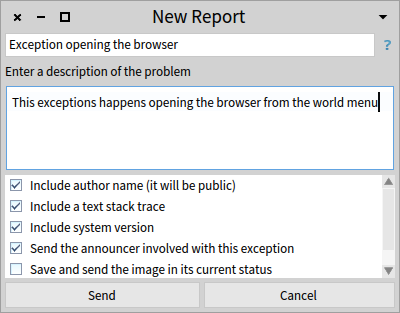
\includegraphics[width=.55\linewidth]{reified/reporter}
  \caption{The reporting window for \sln, where the user can select the data that she wishes to report and add a description}
  \label{fig:reporter}
\end{figure}

In the next section we show how to implement a collector to solve common development problems.


\section{The Framework at Work}\label{sec:reified-stories}

In this section we show how to employ our framework to support debugging and program maintenance.
We present three scenarios and show how to collect domain-specific information from different environments.
We show how accessing specific information can support developers in quickly understanding the cause of a defect and the behavior of a piece of code.

In \secref{sec:reified-story-announcer} we present an in-depth case study together with a possible implementation showing how our approach can support debugging errors in applications using the Announcer framework, a messaging framework that reduces coupling but that might introduce non deterministic behavior; In \secref{sec:reified-story-testing} we outline how to collect data when running a test suite, and how its usage can integrate the current practices in continuous integration of deployed application and support automation; \secref{sec:reified-story-libraries} presents a brief discussion on how using \sln can benefit debugging third party libraries in the context of complex entities.

\subsection{The Announcer Story}\label{sec:reified-story-announcer}

The continuous evolution of the requirements of a software system results in a codebase that grows constantly, both in size and complexity.
To tame this problem, developers design software systems using a modular architecture, where large tasks are split into smaller functionalities, so that complex operations can be managed by composition of small entities, with a defined operational context and limited to few specific responsibilities.
In such a scenario, dispatching messages is fundamental to exchange information among the components and orchestrate the behavior of the modular system.
While the gained modularity is invaluable in developing, testing, and maintaining a system, it comes at a cost: Integrating different modules can show errors generated by the interaction between components and, depending on how the communication is performed, might present non-deterministic behavior.
Since the flow of the execution is distributed into different locations, tracking the source of a defect can become a complicated and time consuming task.
To enable communication among system components, \pha offers the \emph{Announcer} framework: a tool that implements an improved version of the Observer pattern and reduces coupling.
When an entity in the system wants to communicate a message to other entities, it instantiates an \emph{announcer}.
The entities interested in receiving a notifications can then register to the relevant announcer, specifying the type of events they want to observe.
To broadcast a message, a component can create a new \emph{announcement} and send it to the announcer, that dispatches it to the subscribed entities.

The strength of the Announcer framework is that announcements are treated as first class entities: once it occurs, an event is represented by an object that can contain arbitrary data and the subscribers that registered for that event can interact with it using its public interface.
The use of announcements to manage the communications between different applications has numerous advantages, like loosing the coupling between the publisher of an event and its subscribers, and is a recommended best practice in developing an application in \pha.

However, as discussed earlier, fragmenting the control flow of the program into a set of disjoint components carries the drawbacks of event-based programming with the consequence that finding the right fragment of code that is responsible for an error becomes a convoluted process of navigating through the callbacks to find the correct location in the system.
This complicates the debugging process, as understanding how an announcement propagates through the system and affects its status, requires accessing information that is not usually accessible by simply inspecting the stack trace generated by an exception.
The problem with debugging an announcement is that it follows a different logic than the usual sequential style of the rest of the system.
Therefore, while all the information necessary to understand an error is available during an exception, this is usually not exposed by the tools used to catch and report the errors, like the system logger, hence not exploitable to understand and fix the problem.
In particular, to understand an error generated during the broadcasting of an announcement it is not enough to observe the current stack of method calls: As such a structure would only contain information about the subscriber that generated the error, thus hiding the information about the behavior of the other subscribers.
While this might still be sufficient to support debugging of simple problems, it lacks all the collateral information to create the big picture of the status of the announcer and its subscribers.


\subsubsection{Usage of Announcements}

\figref{fig:announcer-report} shows a bug report submitted to the \pha issue tracker, describing a problem with a tool where selection an item from a menu would trigger the opening of two duplicate windows, instead of one.

\begin{figure}[t]
  \centering
  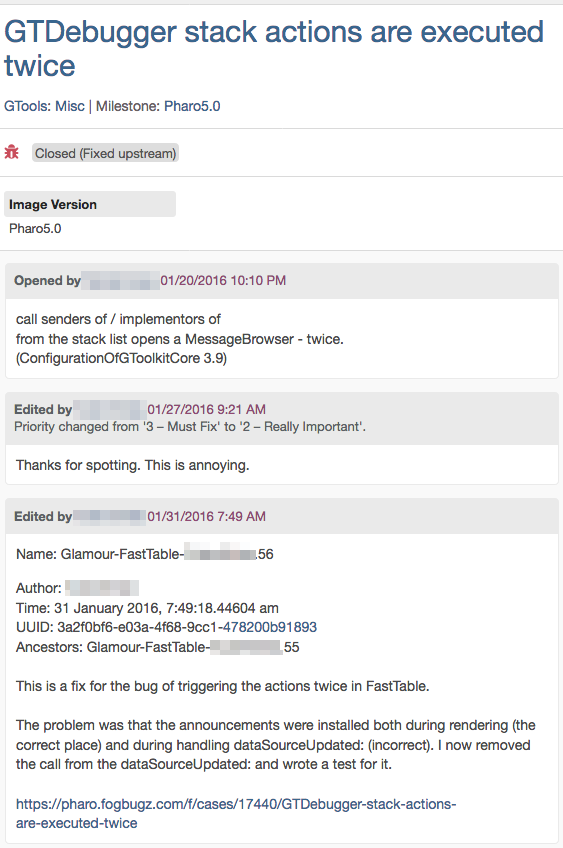
\includegraphics[width=.6\linewidth]{reified/announcer-report-small}
  \caption{A bug report describing a duplicated behavior caused by an entity being registered twice to an announcer}
  \label{fig:announcer-report}
\end{figure}

During the discussion it becomes soon clear that the incident is compatible with the case of an entity registered twice in the announcer responsible for opening the window.
The debugging process consists in hunting down the entity that contains the double registration and remove one of the two snippets of code that perform the subscription.
While this case is not directly a consequence of an exception, it shows how debugging the behavior of code using announcements can be tricky, and that further support from the development tools would probably be preferred.
We therefore conducted a brief experiment to investigate how common are problems involving announcements in the exceptions that developers usually trigger while writing code.

For this purpose, we inspected the data collected through \sln, the tool we presented in \chref{ch:stacktraces} to intercept stack traces from development exceptions and report them to a central server to support debugging~\cite{DalS2015a}.
We considered the stack traces collected from 10 June 2014 to 28 February 2017.
\tabref{tab:stack-traces} shows a summary of the collected data.

\begin{table}[h]
\centering
\caption{Summary of the collected stack trace data}
\begin{tabular}{lr}
\hline
Oldest stack trace & 10 June 2014 \\
Newest stack trace & 28 February 2017 \\
\# of days & 994\\
\# of developers & 257\\
average \# of traces per day & $\sim$41\\
\# of stack traces & 41,129 \\
\# of traces involving announcements & 4,840 \\
\% of traces involving announcements & $\sim$12\% \\
\hline
\end{tabular}
\label{tab:stack-traces}
\end{table}


The collecting tool can be set to submit every exception automatically, or to ask the developer whether she wants to explicitly submit it.
The stack traces collected come from exceptions generated by users of the \pha platform from their daily development activities.
We collected 41,129 stack traces from 257 different developers, on a time period of almost three years.
We queried the collected data looking for references to \textit{AnnouncementSubscription}, the class responsible to dispatch the announcement to the registered entities, and we found that 4,840 stack trace contain at least one reference to this class.

Such a result means that almost 12\% of the exceptions that were collected by our tool as a result of a system exception, involved the usage of the Announcement framework.
While this result does not imply that the framework is directly responsible or involved with the error, it shows that more than one exception every ten has in its source a relation with an announcement.
This hints that the scenario is frequent enough to require a dedicated support by the debugging tools, not only to correct errors, but also to help understanding the status of the system during its execution.


\subsubsection{Implementation of the collector}

Our goal is to use a model able to collect and present domain-specific information about the message dispatching.
We can use this information to refine the inspection tools used to investigate the system, or to create bug reports capable of representing the exception with further details that are not representable using the stack trace generated by the exception.

We can accomplish the task using a custom extension of \sln to collect runtime data that describes the environment of an announcement.
To implement the collector we need to define the strategies to activate for its activation and to describe the data extraction.
There are two main scenarios that can lead to errors using an announcer: \figref{fig:announcer-report} showed how an entity being registered twice to an announcer can lead to weird bugs, while the potentially non-deterministic nature of an announcer, given by the fact that messages are dispatched in no specific order, can cause bugs that are hard to reproduce.
We therefore decide to observe four features:
%
\begin{inparaenum}[(1)]
  \item the subscribers of the announcer listening for the specific announcement,
  \item the announcement being dispatched,
  \item the subscriber that generated the exception, and
  \item the list of subscribers that already received the announcement compared to the list of subscribers that did not receive it yet.
\end{inparaenum}
%
\figref{fig:announcer-code} shows the implementation of \textit{AnnouncerCollector} the class responsible for gathering data about an announcement.

\begin{figure}[t]
\centering
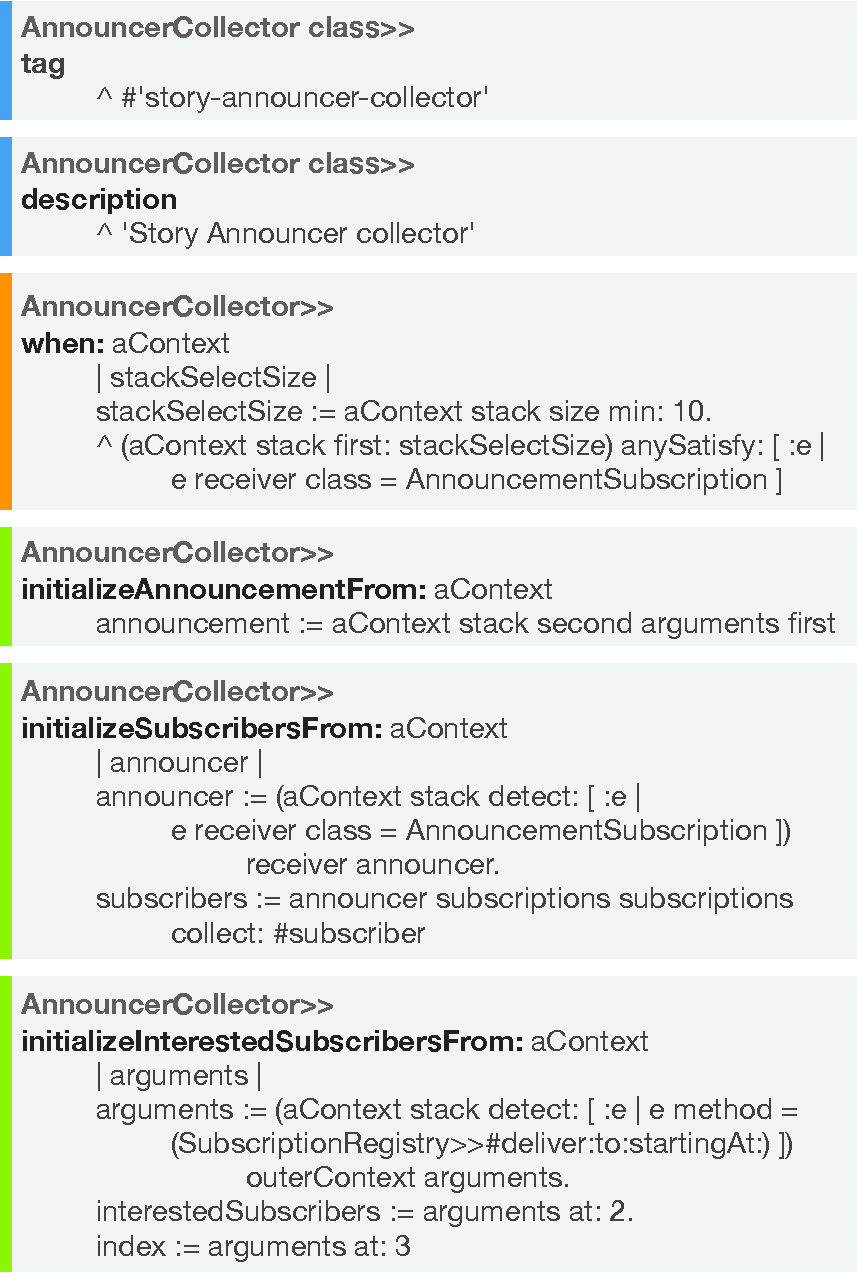
\includegraphics[width=.6\linewidth]{reified/announcer-collector}
\caption{The Smalltalk code implementing the extraction strategies for the Announcer collector}
\label{fig:announcer-code}
\end{figure}

The methods \method{\#tag} and \method{\#description}, from the class side of AnnouncerCollector describe the collector, for indexing and user interaction purposes.
The method \method{\#when:} checks the current context object and verifies if there is a reference to a \entity{AnnouncementSubscription} object in the first 10 lines of the method invocation stack, to ensure that announcements are involved in the exceptions in the immediate surroundings of the current context.
The other three methods are invoked during the initialization of the collector, once the \method{\#when:} returned a positive response:
\method{\#initializeAnnouncementFrom:} extracts the information of the announcement that triggered the broadcasting process, together with possible data that it was supposed to deliver;
\method{\#initializeSubscribersFrom:} extracts all the entities registered to the announcer, regardless of the kind of announcement they are listening to;
\method{\#initializeInterestedSubscribersFrom:} extracts the distribution list of the announcer.
Since this data is collected during the execution time, this list contains the order in which this announcement is being distributed.
Moreover, the method also extracts the index of the current entity: In this way the developer can access the list of the entities that already received the announcement and the one of the entities that did not receive the message, thus easing the detection of possible conflicts between different subscribers.

The data collected by the Announcer collector provides a detailed picture of the status of a program, in an environment where it is usually hard to understand what causes the code to fail, thus giving the developer an immediate overlook on the dispatching of the messages.
Moreover, the data collected are still first-class entities of the system, that can be further queried to extract data: this process allows to retain the maximum amount of information for the longest time needed, so that it can be inspected during an exception or flattened into a textual format for the submission to an issue tracking system.
If the system allows it, the entities can also be serialized and sent to the issue tracker, so that the maintainers of a software can navigate the errors generated by the users with a much higher degree of flexibility and introspection on the data than just plain text log files.

Stepping aside from the specific case of the announcer, this example shows how our framework can help developers to easily extend the behavior of the logging mechanism to collect domain-specific data that pertains to the software they develop.
By distributing a software together with some custom collectors, a developer can effortlessly select the exceptions that are caused by her software, collect relevant data ---with the consent of the user--- and browse it to debug the error.

\subsection{The Testing Story}\label{sec:reified-story-testing}
%Collectors can be put in place to refine and augment test execution, impacting the way we conduct tests both in an interactive fashion or automatically with a continuous integration server.

Bug fixing is an essential part of software development: Therefore, part of the development effort consists in ensuring that a piece of code behaves in the intended way as the codebase changes.
The main tool for this purpose is represented by unit and integration tests, that help the developers to immediately spot unexpected behaviors and locate the responsible components.
The use of test cases plays a central role in developing software, especially since the advent of agile techniques like \emph{Test Driven Development} (TDD) and continuous integration~\cite{Beck2001manifesto}.
The former expects the developer to write a test mapping the expected outcome before writing the code to perform the task, while the latter consists in automating the testing process by integrating it in the development workflow.

We analyze the possible role of our approach based on collectors within the combination of these two specific contexts.
While in the case of TDD the developer has immediate access to the error and its context, running a test suite to check the whole codebase can generate errors that are complex to frame in the correct context.
Moreover, in the case of continuous integration, where the tests do not run on the machine of the developer but are executed on a remote server, developers only have access to the output of the tests, which usually consist on textual reports.
This happens for example if a project adopts a continuous integration service like Travis CI,\seeurl{https://travis-ci.org/} that performs a full run of the tests every time the project is updated, and then sends a report of the outcome to the developers.

When a test fails, however, the trace of the error is flooded into the log messages generated during the build process, requiring time to identify and filter the relevant information.
Once a developer finds information about the failed test, she has to read the text output to understand what was the possible cause of the failure, return to her development environment, reproduce the failed case, locate the source of the defect and fix it.
This process might still be lightweight in the case of simple defects in small projects with one developer, but as the organization of the project grows in complexity, reproducing and locating the issue can become a burden that costs a significant amount of time.
We can improve this scenario by introducing \sln collectors.
By writing a small amount of code, developers are able to extract the specific information they are interested in about a failing test.
Writing a collector for a test case is simple: Smalltalk uses the testing suite called \textit{SUnit}~\cite{Beck1994a}, where each test class is a subclass of \textit{TestCase}.
We can therefore define the \textit{\#when:} method to activate the collector if there is an instance of such class in the invocation stack of the exception.
We can then write the extraction strategies to gather the status of the part of the system that is subject of the testing, or simply extract the whole context storing all the objects in the stack.

Using collectors, our framework allows developers to generate automatic reports that can be sent and managed in an automated fashion, guaranteeing the reliability and quality of the data.
This data can then be serialized using a framework like \textit{STON},\seeurl{https://github.com/svenvc/ston} so that a developer can still access part of the objects involved with the exception.
The use of objects allows to directly communicate with the status, without having to revert to text mining techniques to infer the involved entities from textual logs.

For example, when a test fails, \entity{SUnit} generates an \entity{AssertionFailure} exception.
Catching this exception allows to access the context of the test, containing the erroneous result and the local variables, especially the class that is object of the test.
By serializing and sending this information, we can collect and group this data from all the failed test to generate an automatic report containing all the objects in a wrong state, and navigate it to identify the cause for the failing tests.

%There is a drawback in customizing collectors to detect specific information in test suites: It is not always possible to define a strategy that is specific enough to collect relevant information, but at the same time broad enough to not require writing a collector for each test case, which would clearly be unfeasible.
Sometimes, however, observing just the tested object is not enough: The cause of the failure might be hidden in the underlying system, or the object would reference volatile resources, like database connections or remote sockets.
In this case we can adopt a different approach and offer a default option to cover the most difficult cases.
Leveraging the Smalltalk approach of the \emph{image}, that can be frozen and saved in a particular state and later reopened with the exact same state, we can write a collector that, when an exception occurs, saves the image and sends it to a central server with a report containing metadata about the exception.
Using this approach, when a build fails to pass the tests, the developer can browse the repository of images, download the relevant one and open it on its local machine.
The concept is similar to using \emph{Docker}\footnote{\url{https://www.docker.com/}} to deploy applications, where the system runs in an isolated controlled environment, independent from the host operating system.

Either using the automatic report generated by the failing tests, or downloading directly the image containing the error, developers can observe details of the system at the moment of the failure, thus shortening the time required to identify the steps to reproduce the error, and reduce the maintenance cost.

\subsection{Debugging Third Party Libraries}\label{sec:reified-story-libraries}

The last example on the usage of the framework shows how a developer of a third party library can benefit from implementing a collector observing for specific data about her project.
In the Smalltalk ecosystem, \emph{Roassal}\footnote{\url{http://agilevisualization.com/}} is a large and vastly used visualization engine made to ``visualize and interact with arbitrary data, defined in terms of objects and their relationships''~\cite{Aray2013a}.
Roassal codebase consists of more than 800 classes and almost 6,000 methods, and is constantly evolving and improving using the feedback of the community.
Maintaining such a large project is a complicated task, as tracing and addressing the errors experienced by the users can become like hitting a moving target, especially since Roassal integrates with other tools and because the community is usually split among stable, legacy, and development releases.

Understanding what triggered an error and rebuilding the environment to reproduce it can become quite painful, as the developers need information that might not be easy to provide.
Using a coarse-grained approach as the one we described in \secref{sec:reified-story-testing} would not fit this scenario, as asking the user to submit the whole image would generate a lot of traffic that would be hard to manage, without considering that the image could contain sensitive data, like private source code, that a user might not want to share.

The maintainers of Roassal can improve this situation by observing data specifically related the the model of the engine.
By detecting either when an exception occurs involving an object that is a subclass of \textit{RTObject}, or by checking if it happens in the context of a builder ---a Roassal object responsible for generating a visualization from a collection of data---, a collector can determine if there is some information about Roassal available, that can be collected and reported.

By collecting domain-specific information, the maintainers can get a much more detailed picture of the error, and restrict the possible causes to the ones compatible with the collected data without the need to access the actual data of the user.
For example, by knowing the number of nodes that a visualization is rendering, one could tell if the error is due to a memory problem, or if the visualization has scalability issues.
Instead, knowing the settings that were used to configure a builder can tell if there is a bug in the builder's code, or if the public API is poorly designed and therefore often misused by the users.
Finally, knowing the kind of data that a visualization received can help in finding if there is a bug in managing objects of different (specific) types.

By shipping their own collectors for observing their code, developers can support debugging in the context of the project, therefore reducing the time required to understand an error and lowering the cost for maintenance.


\section{Summary}\label{sec:reified-summary}

We presented an approach to define ad-hoc collection of runtime data to support debugging.
By extending our framework, a developer can define a custom strategy to gather domain-specific knowledge that follows the model of the application she wants to observe.
By preserving the structured, object-oriented nature of the collected data, rather than serializing the information to text, we are able to query the state of a program  and observe it by filtering the data we are interested in, resulting in both more expressive and less bloated reports.
Such capabilities of observing a system enable to create flexible inspection tools, that are able to get a deeper representation of the execution context of a piece of software.

By giving the possibility to report and collect specific information from the system, \sln offers data that is more reliable that a stack trace submitted by a user, and allows to deal with the collected data in an automated fashion, giving the possibility to programmatically perform tasks that would otherwise consume time of the developers and weight on the cost of maintenance.
Moreover, providing a defined structure for execution data, our framework allows to perform a number of analyses without having to resort to information retrieval and text mining techniques to clean the data, but allows to talk directly with the collected entities that map the original data.

Finally, dealing with data that is not flattened allows to perform a progressive inspection of a report, enabling the discoverability of complex data and structuring the debugging session as a browsing process to select the data needed by the developer fixing a bug.


\subsubsection{Generalizability of the approach}

As we explained in \chref{ch:pharo}, we developed our approach using \pha.
The strong reflection and inspection capabilities of the platform allowed us to inspect the whole status of the system, retrieving valuable information about the whole execution context of the software.

Given these premises, one might wonder (1) why should this approach be relevant in the \pha ecosystem, and (2) if it is still relevant outside \pha, when trying to apply it to other programming languages.

To answer question (1), this framework comes after a long collaboration with the \pha community, to understand the types of errors that users get during the use and the development of the platform.
As we discussed through the chapter, the data collection mechanism can be integrated with the issue tracking system of a project, allowing the developers of a project to integrate \sln in their workflow, supporting debugging and maintenance tasks.
About question (2), we believe that it is possible to implement such an approach also in other programming languages.
The \pha system makes the perfect candidate to test such a framework, easing the implementation process by providing the APIs to talk with the system and the tools to navigate the collected data, but the use cases we have shown in \secref{sec:reified-stories} can be implemented with any language with reflective capabilities.

There is also an interesting aspect to consider pertaining to how we used a collector in section \secref{sec:reified-story-testing} to save and submit the whole \pha image.
Given the current interest in DevOps technologies like Docker\footnote{\url{https://www.docker.com/}}, it is possible to execute an application in a Docker container, stop it and save its status during an exception, and submit the image of the application to a remote server.
Analyzing the stored data would not be simple, as there is a lack of tools to access the state of applications in these circumstances, but our approach could be an interesting match for these similar scenarios.


\subsection{Next Steps}

Building collectors to observe specific parts of the system can improve the workflow of debuggers, and reduce maintenance costs.
The regular collection of domain-specific data can provide statistics on the frequency of errors in selected parts of the system, and hint how the users use a software, hence helping developers not only to debug a system, but also to optimize the existing code and improve the API.
%We plan to propose \sln for the integration with the next standard \pha distribution, proposing some generic collectors to support standard difficult debugging tasks, like the one that we proposed in \secref{sec:reified-story-announcer} about the Announcer framework.
%By reaching a larger user base we can collect more specific data about the usage of the tool, refine further the collectors implementation and evaluate the impact of such an approach in daily development activities.

We envision a future where development activities are supported by the system using the language of the system, not resolving to flat and bloated chunks of plain text that represent the side effects of the code, but rather first-class entities that narrate the exact status of a program.
Starting a conversation with the entities we can develop a paradigm of programming that focuses on the models and their interactions, rather than manipulating strings, and achieve a programming environment that is really live and responsive.


\subsubsection{The Road So Far...}

In this chapter we put in place a platform to collect detailed domain-specific information about components of a system.
In the next chapter we present an approach to employ the information collected about a system in a tool for browsing the history and the evolution of a software system.
